% Options for packages loaded elsewhere
\PassOptionsToPackage{unicode}{hyperref}
\PassOptionsToPackage{hyphens}{url}
%
\documentclass[
]{book}
\usepackage{amsmath,amssymb}
\usepackage{lmodern}
\usepackage{ifxetex,ifluatex}
\ifnum 0\ifxetex 1\fi\ifluatex 1\fi=0 % if pdftex
  \usepackage[T1]{fontenc}
  \usepackage[utf8]{inputenc}
  \usepackage{textcomp} % provide euro and other symbols
\else % if luatex or xetex
  \usepackage{unicode-math}
  \defaultfontfeatures{Scale=MatchLowercase}
  \defaultfontfeatures[\rmfamily]{Ligatures=TeX,Scale=1}
\fi
% Use upquote if available, for straight quotes in verbatim environments
\IfFileExists{upquote.sty}{\usepackage{upquote}}{}
\IfFileExists{microtype.sty}{% use microtype if available
  \usepackage[]{microtype}
  \UseMicrotypeSet[protrusion]{basicmath} % disable protrusion for tt fonts
}{}
\makeatletter
\@ifundefined{KOMAClassName}{% if non-KOMA class
  \IfFileExists{parskip.sty}{%
    \usepackage{parskip}
  }{% else
    \setlength{\parindent}{0pt}
    \setlength{\parskip}{6pt plus 2pt minus 1pt}}
}{% if KOMA class
  \KOMAoptions{parskip=half}}
\makeatother
\usepackage{xcolor}
\IfFileExists{xurl.sty}{\usepackage{xurl}}{} % add URL line breaks if available
\IfFileExists{bookmark.sty}{\usepackage{bookmark}}{\usepackage{hyperref}}
\hypersetup{
  hidelinks,
  pdfcreator={LaTeX via pandoc}}
\urlstyle{same} % disable monospaced font for URLs
\usepackage{color}
\usepackage{fancyvrb}
\newcommand{\VerbBar}{|}
\newcommand{\VERB}{\Verb[commandchars=\\\{\}]}
\DefineVerbatimEnvironment{Highlighting}{Verbatim}{commandchars=\\\{\}}
% Add ',fontsize=\small' for more characters per line
\usepackage{framed}
\definecolor{shadecolor}{RGB}{248,248,248}
\newenvironment{Shaded}{\begin{snugshade}}{\end{snugshade}}
\newcommand{\AlertTok}[1]{\textcolor[rgb]{0.94,0.16,0.16}{#1}}
\newcommand{\AnnotationTok}[1]{\textcolor[rgb]{0.56,0.35,0.01}{\textbf{\textit{#1}}}}
\newcommand{\AttributeTok}[1]{\textcolor[rgb]{0.77,0.63,0.00}{#1}}
\newcommand{\BaseNTok}[1]{\textcolor[rgb]{0.00,0.00,0.81}{#1}}
\newcommand{\BuiltInTok}[1]{#1}
\newcommand{\CharTok}[1]{\textcolor[rgb]{0.31,0.60,0.02}{#1}}
\newcommand{\CommentTok}[1]{\textcolor[rgb]{0.56,0.35,0.01}{\textit{#1}}}
\newcommand{\CommentVarTok}[1]{\textcolor[rgb]{0.56,0.35,0.01}{\textbf{\textit{#1}}}}
\newcommand{\ConstantTok}[1]{\textcolor[rgb]{0.00,0.00,0.00}{#1}}
\newcommand{\ControlFlowTok}[1]{\textcolor[rgb]{0.13,0.29,0.53}{\textbf{#1}}}
\newcommand{\DataTypeTok}[1]{\textcolor[rgb]{0.13,0.29,0.53}{#1}}
\newcommand{\DecValTok}[1]{\textcolor[rgb]{0.00,0.00,0.81}{#1}}
\newcommand{\DocumentationTok}[1]{\textcolor[rgb]{0.56,0.35,0.01}{\textbf{\textit{#1}}}}
\newcommand{\ErrorTok}[1]{\textcolor[rgb]{0.64,0.00,0.00}{\textbf{#1}}}
\newcommand{\ExtensionTok}[1]{#1}
\newcommand{\FloatTok}[1]{\textcolor[rgb]{0.00,0.00,0.81}{#1}}
\newcommand{\FunctionTok}[1]{\textcolor[rgb]{0.00,0.00,0.00}{#1}}
\newcommand{\ImportTok}[1]{#1}
\newcommand{\InformationTok}[1]{\textcolor[rgb]{0.56,0.35,0.01}{\textbf{\textit{#1}}}}
\newcommand{\KeywordTok}[1]{\textcolor[rgb]{0.13,0.29,0.53}{\textbf{#1}}}
\newcommand{\NormalTok}[1]{#1}
\newcommand{\OperatorTok}[1]{\textcolor[rgb]{0.81,0.36,0.00}{\textbf{#1}}}
\newcommand{\OtherTok}[1]{\textcolor[rgb]{0.56,0.35,0.01}{#1}}
\newcommand{\PreprocessorTok}[1]{\textcolor[rgb]{0.56,0.35,0.01}{\textit{#1}}}
\newcommand{\RegionMarkerTok}[1]{#1}
\newcommand{\SpecialCharTok}[1]{\textcolor[rgb]{0.00,0.00,0.00}{#1}}
\newcommand{\SpecialStringTok}[1]{\textcolor[rgb]{0.31,0.60,0.02}{#1}}
\newcommand{\StringTok}[1]{\textcolor[rgb]{0.31,0.60,0.02}{#1}}
\newcommand{\VariableTok}[1]{\textcolor[rgb]{0.00,0.00,0.00}{#1}}
\newcommand{\VerbatimStringTok}[1]{\textcolor[rgb]{0.31,0.60,0.02}{#1}}
\newcommand{\WarningTok}[1]{\textcolor[rgb]{0.56,0.35,0.01}{\textbf{\textit{#1}}}}
\usepackage{longtable,booktabs,array}
\usepackage{calc} % for calculating minipage widths
% Correct order of tables after \paragraph or \subparagraph
\usepackage{etoolbox}
\makeatletter
\patchcmd\longtable{\par}{\if@noskipsec\mbox{}\fi\par}{}{}
\makeatother
% Allow footnotes in longtable head/foot
\IfFileExists{footnotehyper.sty}{\usepackage{footnotehyper}}{\usepackage{footnote}}
\makesavenoteenv{longtable}
\usepackage{graphicx}
\makeatletter
\def\maxwidth{\ifdim\Gin@nat@width>\linewidth\linewidth\else\Gin@nat@width\fi}
\def\maxheight{\ifdim\Gin@nat@height>\textheight\textheight\else\Gin@nat@height\fi}
\makeatother
% Scale images if necessary, so that they will not overflow the page
% margins by default, and it is still possible to overwrite the defaults
% using explicit options in \includegraphics[width, height, ...]{}
\setkeys{Gin}{width=\maxwidth,height=\maxheight,keepaspectratio}
% Set default figure placement to htbp
\makeatletter
\def\fps@figure{htbp}
\makeatother
\setlength{\emergencystretch}{3em} % prevent overfull lines
\providecommand{\tightlist}{%
  \setlength{\itemsep}{0pt}\setlength{\parskip}{0pt}}
\setcounter{secnumdepth}{5}
\usepackage{booktabs}
\ifluatex
  \usepackage{selnolig}  % disable illegal ligatures
\fi
\usepackage[]{natbib}
\bibliographystyle{apalike}

\author{}
\date{\vspace{-2.5em}}

\begin{document}

{
\setcounter{tocdepth}{1}
\tableofcontents
}
\hypertarget{resumen}{%
\chapter{Resumen}\label{resumen}}

Este bookdown fue diseñado para ser presentado en la cuarta clase del ramo \emph{Ciencias Sociales Computacionales: Análisis de Redes Sociales y Procesamiento de Lenguaje Natural}, impartida por el profesor Naim Bro Khomasi el segundo semestre del 2021.

\textbf{Curso:} Ciencias Sociales Computacionales - \emph{Análisis de Redes Sociales y Procesamiento de Lenguaje Natural}.\\
\textbf{Institución:} Universidad de Chile.\\
\textbf{Profesor:} Naim Bro Khomasi.\\
\textbf{Ayudantes:} Jan Dimter y Nicolas Godoy.\\
\textbf{Fecha:} 26 de agosto de 2021.

\hypertarget{introducciuxf3n-clase}{%
\chapter{Introducción clase}\label{introducciuxf3n-clase}}

En esta clase realizaremos ejercicios de visualización a través de las librerías \textbf{ggplot2} y \textbf{plotly}. Utilizaremos el dataset \texttt{mpg} para la creación de gráficos. Éste se encuentra contenido en \emph{tidyverse} \footnote{Esta librería llama paquetes adicionales del universo tidyverse tales como ggplot2, dplyr, readr, stringr, etc.}\emph{.}

Realizamos la instalación y carga de los paquetes con el siguiente código:\\

\begin{Shaded}
\begin{Highlighting}[]
\CommentTok{\#install.packages("tidyverse")}
\CommentTok{\#install.packages("plotly")}
\FunctionTok{library}\NormalTok{(tidyverse)}
\FunctionTok{library}\NormalTok{(plotly)}
\end{Highlighting}
\end{Shaded}

\hypertarget{sobre-el-dataset}{%
\section{Sobre el dataset}\label{sobre-el-dataset}}

Según la documentación de mpg (puedes encontrarla usando en tu consola el comando \texttt{?mpg} una vez hayas instalado ggplot2), las variables son las siguientes:

\begin{longtable}[]{@{}
  >{\centering\arraybackslash}p{(\columnwidth - 2\tabcolsep) * \real{0.18}}
  >{\raggedright\arraybackslash}p{(\columnwidth - 2\tabcolsep) * \real{0.82}}@{}}
\toprule
Variable & Detalle \\
\midrule
\endhead
\textbf{manufacturer} & Marca del auto \\
\textbf{model} & Modelo del auto \\
\textbf{displ} & Cilindrada, en litros. \\
\textbf{year} & Año de manufactura \\
\textbf{cyl} & Número de cilindros \\
\textbf{trans} & Tipo de transmisión \\
\textbf{drv} & Tipo de transmisión (f = transmisión delantera, r = transmisión trasera, 4 = 4x4) \\
\textbf{cty} & Millas por galón en ciudad \\
\textbf{hwy} & Millas por galón en autopista \\
\textbf{fl} & Tipo de combustible \\
\textbf{class} & Tipo de auto \\
\bottomrule
\end{longtable}

Una vez cargados los paquetes, revisamos las primeras y últimas filas de nuestro dataset:

\begin{Shaded}
\begin{Highlighting}[]
\CommentTok{\# Usamos knitr::kable() para ajustar el resultado a la visualización html.}
\CommentTok{\# Una alternativa más simple es usar por separadop las funciones head() y tail().}
\NormalTok{knitr}\SpecialCharTok{::}\FunctionTok{kable}\NormalTok{(mpg[}\FunctionTok{c}\NormalTok{(}\DecValTok{1}\SpecialCharTok{:}\DecValTok{3}\NormalTok{,(}\FunctionTok{nrow}\NormalTok{(mpg)}\SpecialCharTok{{-}}\DecValTok{2}\NormalTok{)}\SpecialCharTok{:}\FunctionTok{nrow}\NormalTok{(mpg)),])}
\end{Highlighting}
\end{Shaded}

\begin{tabular}{l|l|r|r|r|l|l|r|r|l|l}
\hline
manufacturer & model & displ & year & cyl & trans & drv & cty & hwy & fl & class\\
\hline
audi & a4 & 1.8 & 1999 & 4 & auto(l5) & f & 18 & 29 & p & compact\\
\hline
audi & a4 & 1.8 & 1999 & 4 & manual(m5) & f & 21 & 29 & p & compact\\
\hline
audi & a4 & 2.0 & 2008 & 4 & manual(m6) & f & 20 & 31 & p & compact\\
\hline
volkswagen & passat & 2.8 & 1999 & 6 & auto(l5) & f & 16 & 26 & p & midsize\\
\hline
volkswagen & passat & 2.8 & 1999 & 6 & manual(m5) & f & 18 & 26 & p & midsize\\
\hline
volkswagen & passat & 3.6 & 2008 & 6 & auto(s6) & f & 17 & 26 & p & midsize\\
\hline
\end{tabular}

\hypertarget{ggplot2-componentes-base}{%
\chapter{ggplot2: Componentes base}\label{ggplot2-componentes-base}}

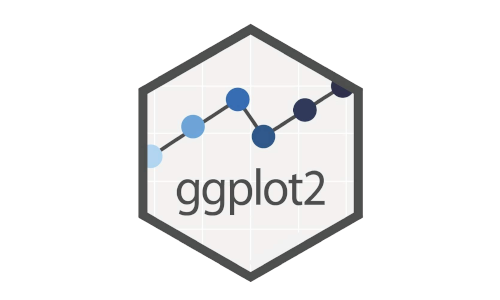
\includegraphics[width=2.08333in,height=\textheight]{Data/ggplot2_logo.png}

La librería ggplot2 de \href{http://hadley.nz/}{Hadley Wickham} et al.~(2014), parte del ecosistema de paquetes \textbf{\emph{tidyverse,}} es un sistema declarativo para la creación de gráficos. ¿Qué quiere decir eso? Que le señalamos a ggplot2 cuál es nuestra data, cómo mapearla, qué elementos gráficos usar, y ggplot se encarga del resto.

\begin{Shaded}
\begin{Highlighting}[]
\FunctionTok{ggplot}\NormalTok{(mpg, }\FunctionTok{aes}\NormalTok{(displ, hwy, }\AttributeTok{colour =}\NormalTok{ class)) }\SpecialCharTok{+} 
  \FunctionTok{geom\_point}\NormalTok{()}
\end{Highlighting}
\end{Shaded}

Son 3 los componentes base a la hora de trabajar con ggplot2:

\begin{enumerate}
\def\labelenumi{\arabic{enumi}.}
\tightlist
\item
  \textbf{Data}: literalmente son los datos que le entregaremos. Comunmente serán \emph{data frames} o similares\emph{.} Pueden estar agrupados o no. En el caso de nuestro ejemplo corresponde a \texttt{mpg}.
\item
  \textbf{Aesthetic mapping:} corresponde a indicadores en torno a la data que usamos. Posiblemente los más comunes e importantes son los parámetros x e y (ej. en un diagrama de dispersión). También podemos incorporar distinción por colores, formas, etc. En nuestra sintaxis de ejemplo, corresponde a \texttt{aes(displ,\ hwy,\ colour\ =\ class)}.
\item
  \textbf{Geometry:} Hasta ahora hemos señalado nuestra data y qué representación le daremos en el gráfico, sin embargo, nos falta el último componente: ¿qué tipo de gráfico usaremos? Es posible generar puntos, barras, cajas, etc. Las geometrías suelen ser combinables dependiendo del tipo de información con la que trabajes. En nuestro código de ejemplo corresponde a \texttt{geom\_point()}.
\end{enumerate}

El resultado de ejemplo es el siguiente:

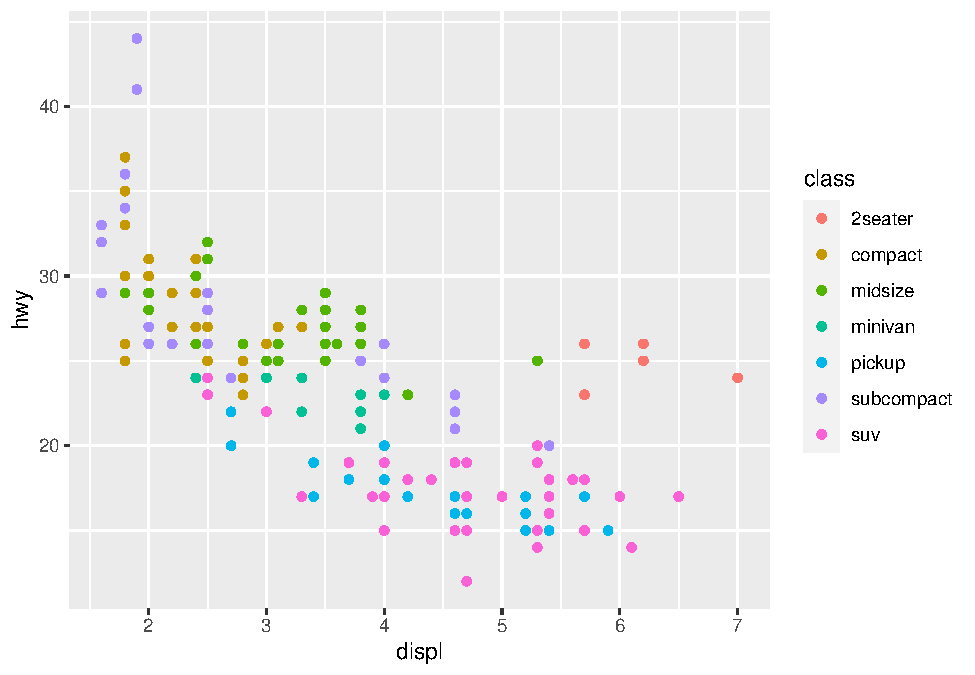
\includegraphics{clase_visualizacion_CSC_files/figure-latex/unnamed-chunk-4-1.pdf}

\hypertarget{ggplot-principales-tipos-de-gruxe1ficos}{%
\chapter{ggplot: Principales tipos de gráficos}\label{ggplot-principales-tipos-de-gruxe1ficos}}

Revisaremos rápidamente gráficos que puedes constuir usando ggplot. Usaremos para este fin mpg.

\begin{enumerate}
\def\labelenumi{\arabic{enumi}.}
\tightlist
\item
  \textbf{Histograma} (histogram)
\end{enumerate}

\begin{Shaded}
\begin{Highlighting}[]
\NormalTok{histograma }\OtherTok{\textless{}{-}} \FunctionTok{ggplot}\NormalTok{(mpg, }\FunctionTok{aes}\NormalTok{(}\AttributeTok{x=}\NormalTok{cty)) }\SpecialCharTok{+} 
  \FunctionTok{geom\_histogram}\NormalTok{()}
\NormalTok{histograma}
\end{Highlighting}
\end{Shaded}

\begin{verbatim}
## `stat_bin()` using `bins = 30`. Pick better value with `binwidth`.
\end{verbatim}

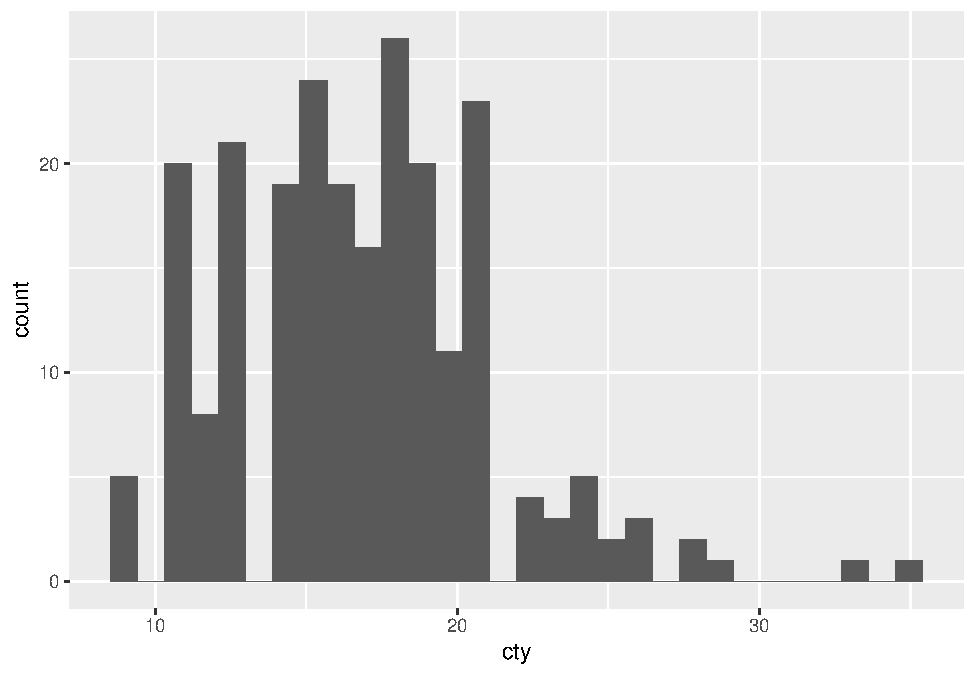
\includegraphics{clase_visualizacion_CSC_files/figure-latex/unnamed-chunk-5-1.pdf}

\begin{enumerate}
\def\labelenumi{\arabic{enumi}.}
\setcounter{enumi}{1}
\tightlist
\item
  \textbf{Gráfico de densidad} (density plot)
\end{enumerate}

\begin{Shaded}
\begin{Highlighting}[]
\NormalTok{densidad}\OtherTok{\textless{}{-}}\FunctionTok{ggplot}\NormalTok{(mpg, }\FunctionTok{aes}\NormalTok{(}\AttributeTok{x=}\NormalTok{cyl))}\SpecialCharTok{+}
  \FunctionTok{geom\_density}\NormalTok{()}
\NormalTok{densidad}
\end{Highlighting}
\end{Shaded}

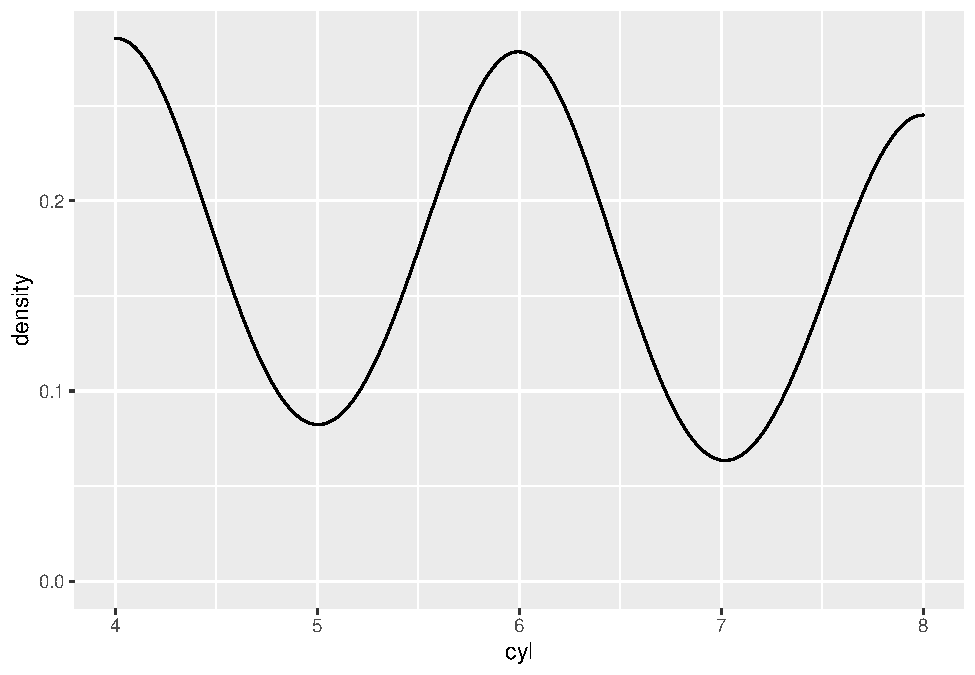
\includegraphics{clase_visualizacion_CSC_files/figure-latex/unnamed-chunk-6-1.pdf}

\begin{enumerate}
\def\labelenumi{\arabic{enumi}.}
\setcounter{enumi}{2}
\tightlist
\item
  \textbf{Diagrama de cajas} (boxplot)
\end{enumerate}

\begin{Shaded}
\begin{Highlighting}[]
\NormalTok{cajas}\OtherTok{\textless{}{-}}\FunctionTok{ggplot}\NormalTok{(mpg, }\FunctionTok{aes}\NormalTok{(}\AttributeTok{x=}\NormalTok{manufacturer, }\AttributeTok{y=}\NormalTok{cty)) }\SpecialCharTok{+} 
    \FunctionTok{geom\_boxplot}\NormalTok{()}
\NormalTok{cajas}
\end{Highlighting}
\end{Shaded}

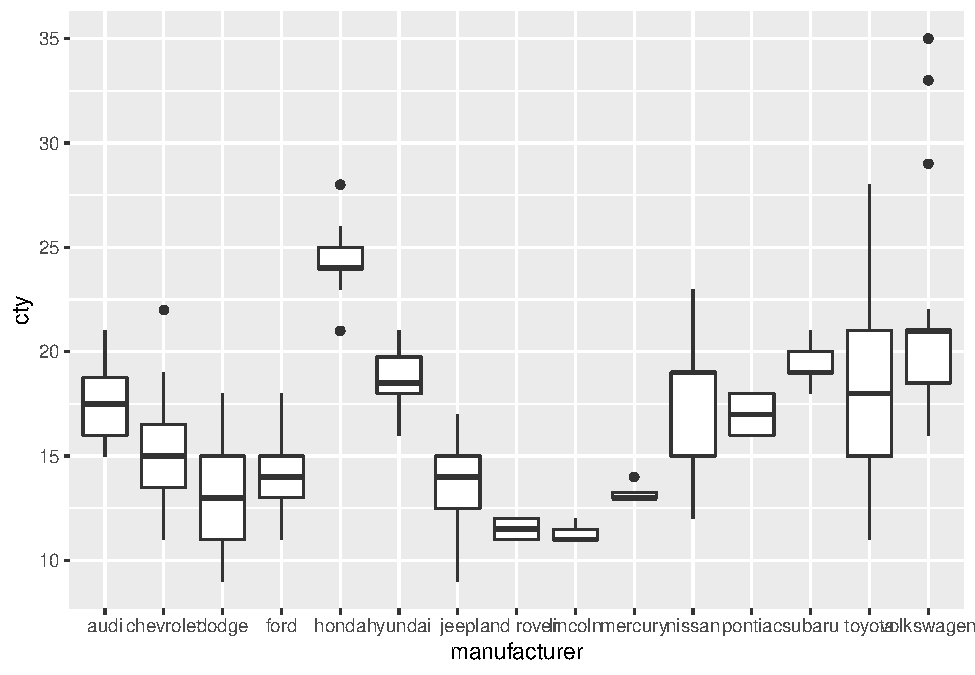
\includegraphics{clase_visualizacion_CSC_files/figure-latex/unnamed-chunk-7-1.pdf}

\begin{enumerate}
\def\labelenumi{\arabic{enumi}.}
\setcounter{enumi}{3}
\tightlist
\item
  \textbf{Diagrama de dispersión} (scatterplot)
\end{enumerate}

\begin{Shaded}
\begin{Highlighting}[]
\NormalTok{dispersion}\OtherTok{\textless{}{-}}\FunctionTok{ggplot}\NormalTok{(mpg, }\FunctionTok{aes}\NormalTok{(}\AttributeTok{x=}\NormalTok{cty, }\AttributeTok{y=}\NormalTok{hwy)) }\SpecialCharTok{+} 
    \FunctionTok{geom\_point}\NormalTok{()}
\NormalTok{dispersion}
\end{Highlighting}
\end{Shaded}

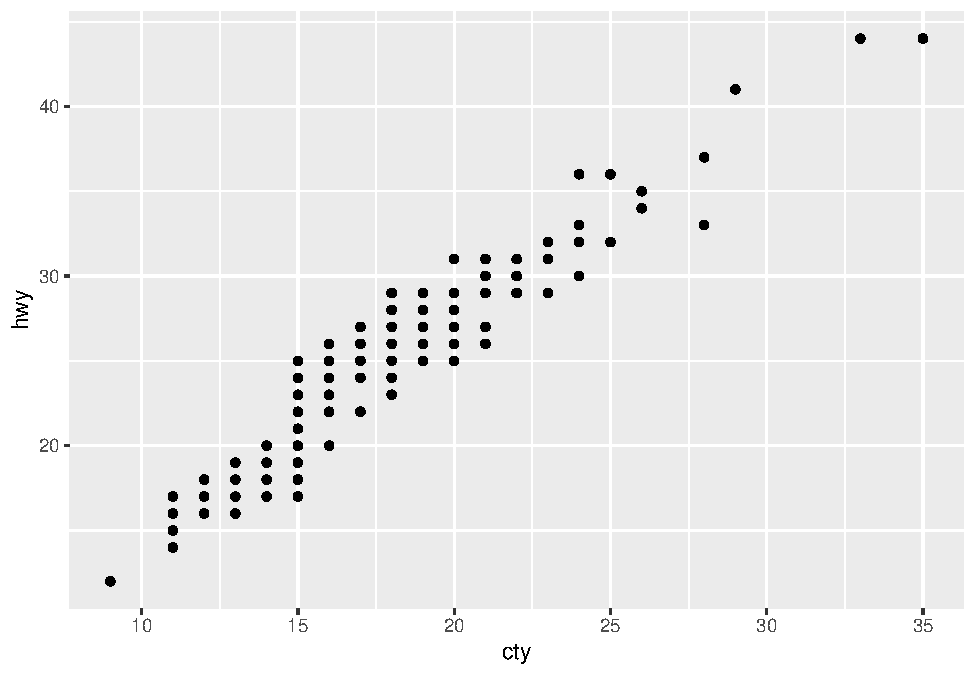
\includegraphics{clase_visualizacion_CSC_files/figure-latex/unnamed-chunk-8-1.pdf}

\begin{enumerate}
\def\labelenumi{\arabic{enumi}.}
\setcounter{enumi}{4}
\tightlist
\item
  \textbf{Gráfico de líneas} (lineplot)
\end{enumerate}

\begin{Shaded}
\begin{Highlighting}[]
\CommentTok{\#Filtramos por un modelo en específico}
\NormalTok{lineas}\OtherTok{\textless{}{-}}\FunctionTok{ggplot}\NormalTok{(mpg[mpg}\SpecialCharTok{$}\NormalTok{model}\SpecialCharTok{==}\StringTok{"range rover"}\NormalTok{,], }\FunctionTok{aes}\NormalTok{(}\AttributeTok{x=}\NormalTok{year, }\AttributeTok{y=}\NormalTok{hwy, }\AttributeTok{group=}\NormalTok{manufacturer)) }\SpecialCharTok{+}
  \FunctionTok{geom\_line}\NormalTok{() }
\NormalTok{lineas}
\end{Highlighting}
\end{Shaded}

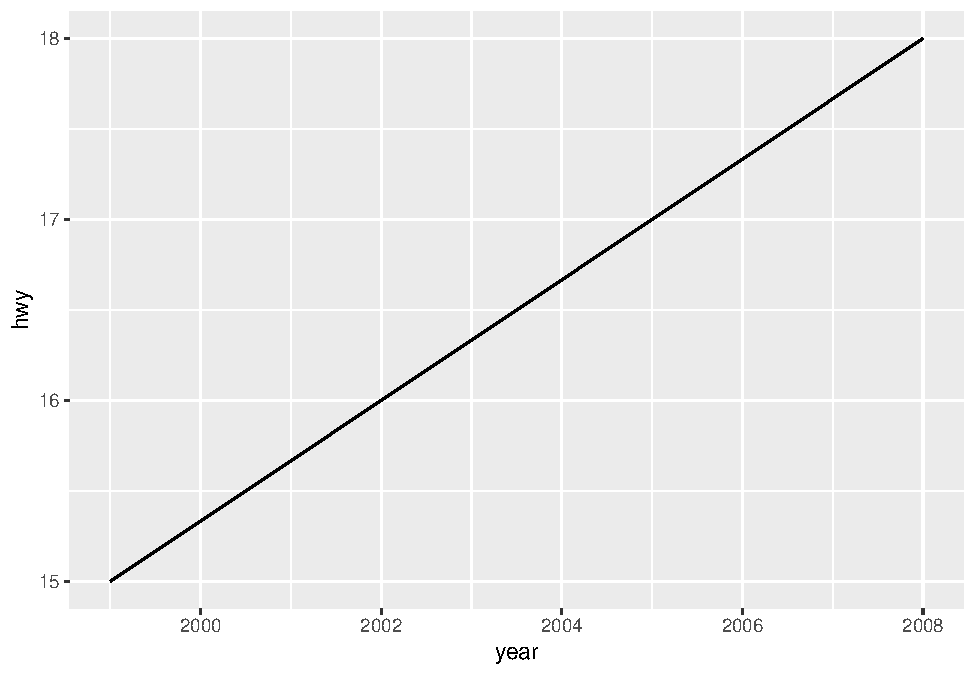
\includegraphics{clase_visualizacion_CSC_files/figure-latex/unnamed-chunk-9-1.pdf}

\hypertarget{intentemos-mejorar-la-visualizaciuxf3n}{%
\section{Intentemos mejorar la visualización}\label{intentemos-mejorar-la-visualizaciuxf3n}}

Si bien los ejemplos anteriores son simples en cuanto a código, la calidad de la visualización es poca. Podemos mejorar los gráficos utilizando argumentos y funciones.

\hypertarget{color}{%
\subsection{Color}\label{color}}

Una gran opción para mejorar nuestros gráficos es incorporar colores. Estos pueden ser iguales para todas las formas como aquí:

\begin{Shaded}
\begin{Highlighting}[]
\NormalTok{histograma }\OtherTok{\textless{}{-}} \FunctionTok{ggplot}\NormalTok{(mpg, }\FunctionTok{aes}\NormalTok{(}\AttributeTok{x=}\NormalTok{cty, }\AttributeTok{fill=}\StringTok{"red"}\NormalTok{)) }\SpecialCharTok{+} 
  \FunctionTok{geom\_histogram}\NormalTok{()}
\NormalTok{histograma}
\end{Highlighting}
\end{Shaded}

\begin{verbatim}
## `stat_bin()` using `bins = 30`. Pick better value with `binwidth`.
\end{verbatim}

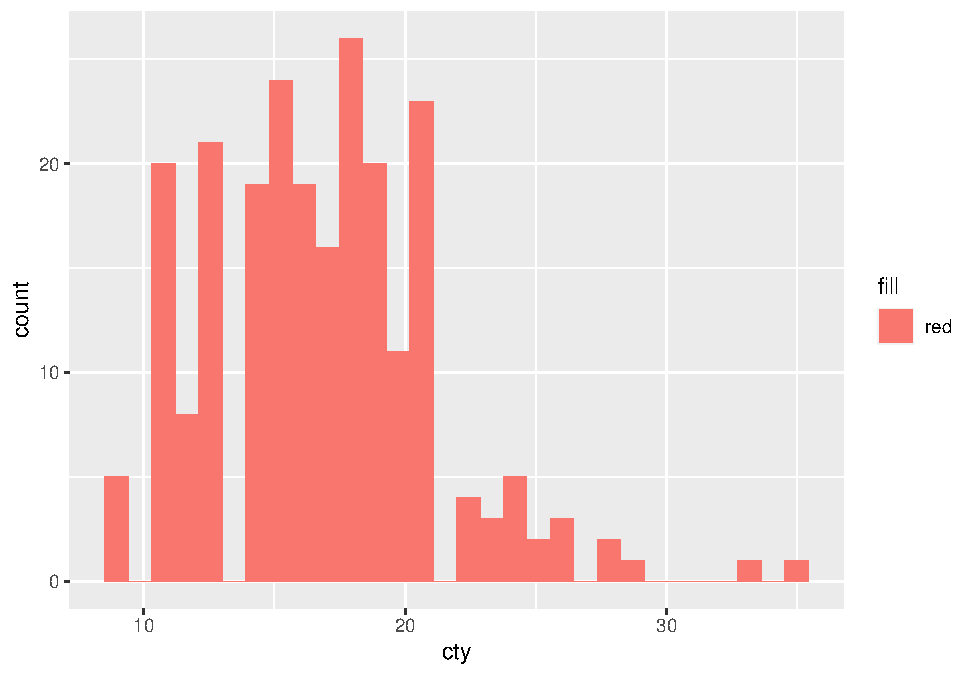
\includegraphics{clase_visualizacion_CSC_files/figure-latex/unnamed-chunk-10-1.pdf}

¿Lo ingresamos correctamente? ¿Es el color de relleno una variable categórica? Lo correcto es incorporarlo como característica de la forma geométrica:

\begin{Shaded}
\begin{Highlighting}[]
\NormalTok{histograma }\OtherTok{\textless{}{-}} \FunctionTok{ggplot}\NormalTok{(mpg, }\FunctionTok{aes}\NormalTok{(}\AttributeTok{x=}\NormalTok{cty)) }\SpecialCharTok{+} 
  \FunctionTok{geom\_histogram}\NormalTok{(}\AttributeTok{fill=}\StringTok{"red"}\NormalTok{)}
\NormalTok{histograma}
\end{Highlighting}
\end{Shaded}

\begin{verbatim}
## `stat_bin()` using `bins = 30`. Pick better value with `binwidth`.
\end{verbatim}

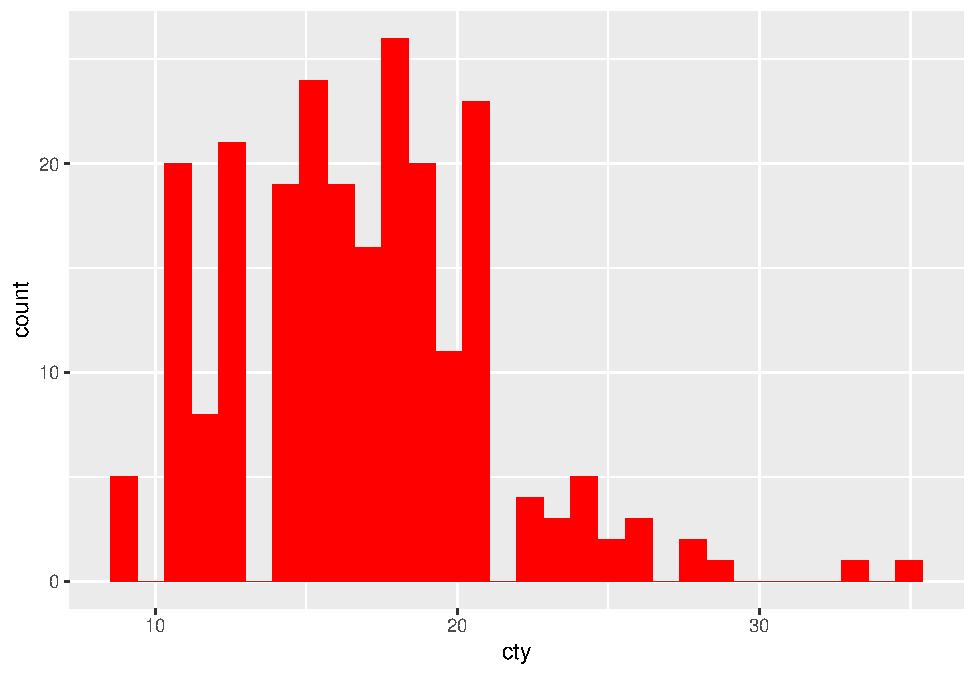
\includegraphics{clase_visualizacion_CSC_files/figure-latex/unnamed-chunk-11-1.pdf}

¿Y si queremos usar los colores para distinguir en relación a una variable categórica? Ahora sí lo incorporamos al mapeo estético:

\begin{Shaded}
\begin{Highlighting}[]
\NormalTok{histograma }\OtherTok{\textless{}{-}} \FunctionTok{ggplot}\NormalTok{(mpg, }\FunctionTok{aes}\NormalTok{(}\AttributeTok{x=}\NormalTok{cty, }\AttributeTok{fill=}\NormalTok{manufacturer)) }\SpecialCharTok{+} 
  \FunctionTok{geom\_histogram}\NormalTok{()}
\NormalTok{histograma}
\end{Highlighting}
\end{Shaded}

\begin{verbatim}
## `stat_bin()` using `bins = 30`. Pick better value with `binwidth`.
\end{verbatim}

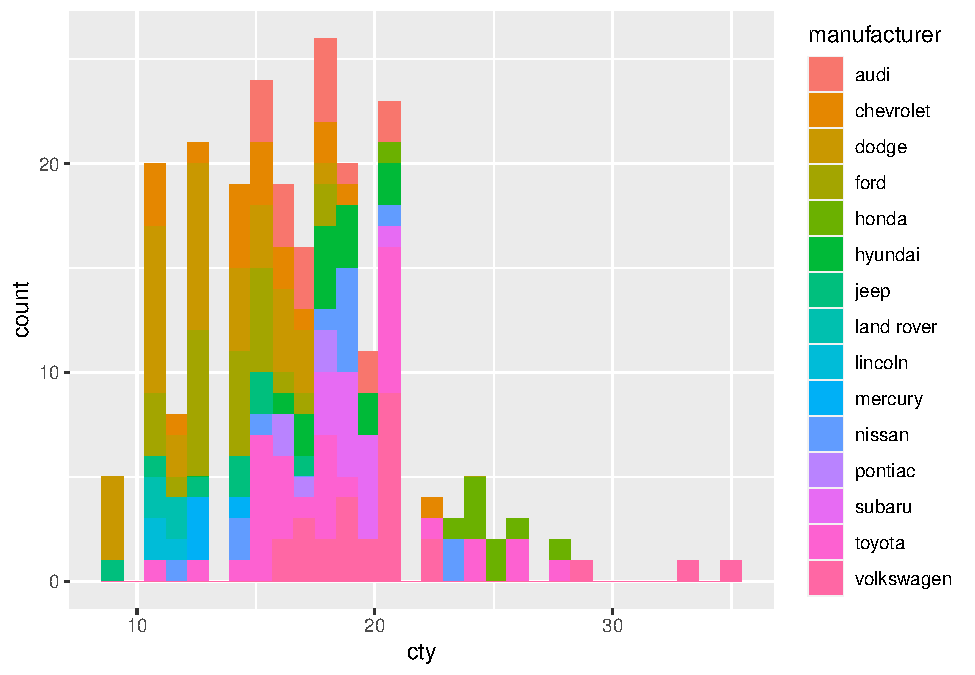
\includegraphics{clase_visualizacion_CSC_files/figure-latex/unnamed-chunk-12-1.pdf}

\hypertarget{formas}{%
\subsection{Formas}\label{formas}}

Al igual que con los colores, podemos personalizar las formas de nuestros gráficos (en particular de nuestros \texttt{geom\_points()}). Para esto modificamos el argumento \texttt{shape}.

\begin{Shaded}
\begin{Highlighting}[]
\NormalTok{dispersion}\OtherTok{\textless{}{-}}\FunctionTok{ggplot}\NormalTok{(mpg, }\FunctionTok{aes}\NormalTok{(}\AttributeTok{x=}\NormalTok{cty, }\AttributeTok{y=}\NormalTok{hwy, }\AttributeTok{shape=}\FunctionTok{as.factor}\NormalTok{(cyl))) }\SpecialCharTok{+} 
    \FunctionTok{geom\_point}\NormalTok{()}
\NormalTok{dispersion}
\end{Highlighting}
\end{Shaded}

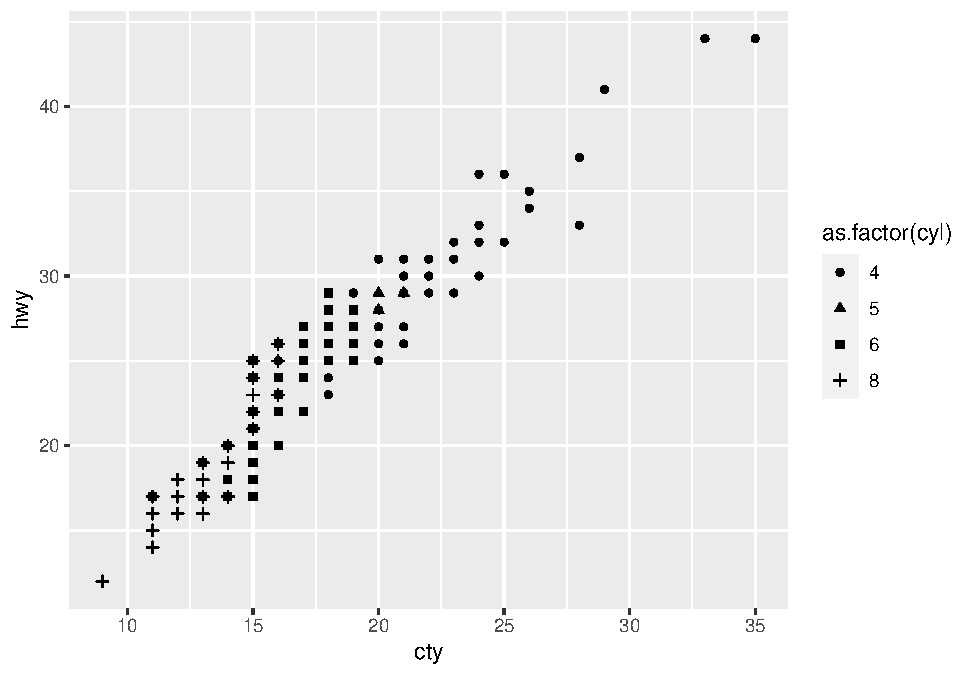
\includegraphics{clase_visualizacion_CSC_files/figure-latex/unnamed-chunk-13-1.pdf}

\hypertarget{tamauxf1o}{%
\subsection{Tamaño}\label{tamauxf1o}}

\begin{Shaded}
\begin{Highlighting}[]
\NormalTok{dispersion}\OtherTok{\textless{}{-}}\FunctionTok{ggplot}\NormalTok{(mpg, }\FunctionTok{aes}\NormalTok{(}\AttributeTok{x=}\NormalTok{manufacturer, }\AttributeTok{y=}\NormalTok{cty, }\AttributeTok{size=}\NormalTok{displ)) }\SpecialCharTok{+} 
    \FunctionTok{geom\_point}\NormalTok{()}
\NormalTok{dispersion}
\end{Highlighting}
\end{Shaded}

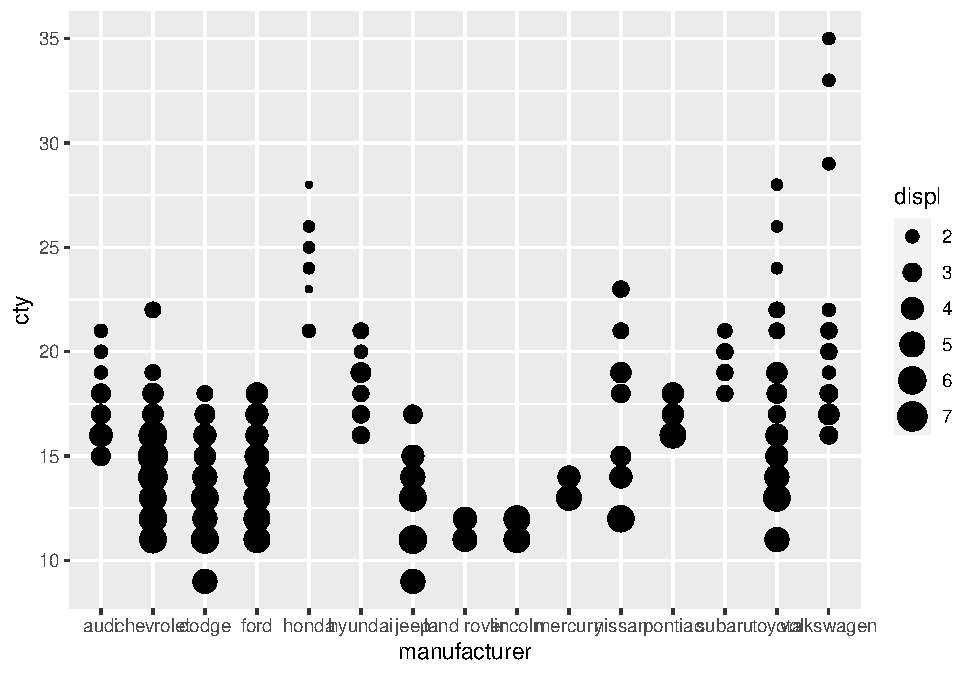
\includegraphics{clase_visualizacion_CSC_files/figure-latex/unnamed-chunk-14-1.pdf}

\hypertarget{mezcluxe9moslas}{%
\subsection{Mezclémoslas}\label{mezcluxe9moslas}}

\begin{Shaded}
\begin{Highlighting}[]
\NormalTok{dispersion}\OtherTok{\textless{}{-}}\FunctionTok{ggplot}\NormalTok{(mpg, }\FunctionTok{aes}\NormalTok{(}\AttributeTok{x=}\NormalTok{manufacturer, }\AttributeTok{y=}\NormalTok{cty, }\AttributeTok{size=}\NormalTok{displ, }\AttributeTok{shape=}\FunctionTok{as.factor}\NormalTok{(year),}\AttributeTok{color=}\FunctionTok{as.factor}\NormalTok{(cyl)))}\SpecialCharTok{+}
  \FunctionTok{geom\_point}\NormalTok{()}
\NormalTok{dispersion}
\end{Highlighting}
\end{Shaded}

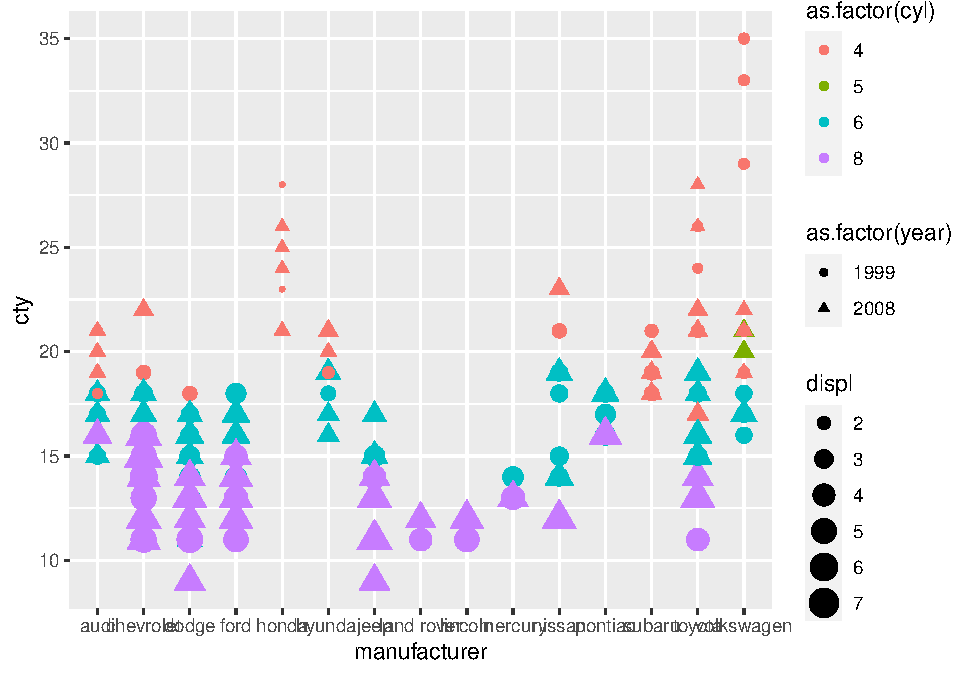
\includegraphics{clase_visualizacion_CSC_files/figure-latex/unnamed-chunk-15-1.pdf}

\hypertarget{orden}{%
\subsection{Orden}\label{orden}}

Podemos utilizar la función reorder() para

\begin{Shaded}
\begin{Highlighting}[]
\NormalTok{cajas}\OtherTok{\textless{}{-}}\FunctionTok{ggplot}\NormalTok{(mpg, }\FunctionTok{aes}\NormalTok{(}\AttributeTok{x=}\FunctionTok{reorder}\NormalTok{(manufacturer, cty, median), }\AttributeTok{y=}\NormalTok{cty)) }\SpecialCharTok{+} 
    \FunctionTok{geom\_boxplot}\NormalTok{()}
\NormalTok{cajas}
\end{Highlighting}
\end{Shaded}

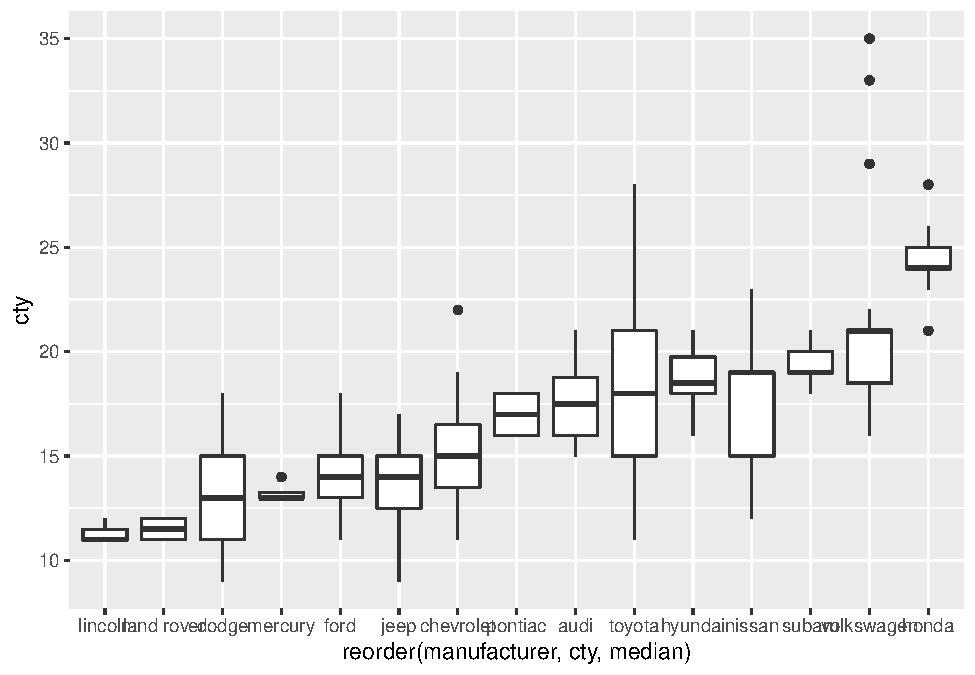
\includegraphics{clase_visualizacion_CSC_files/figure-latex/unnamed-chunk-16-1.pdf}

Para invertir el orden agregamos un guión (``-'') antes del segundo argumento.

\begin{Shaded}
\begin{Highlighting}[]
\CommentTok{\#Creamos datos de ejemplo }
\NormalTok{df }\OtherTok{\textless{}{-}} \FunctionTok{data.frame}\NormalTok{(}\AttributeTok{nombres =} \FunctionTok{c}\NormalTok{(}\StringTok{"a"}\NormalTok{, }\StringTok{"b"}\NormalTok{, }\StringTok{"c"}\NormalTok{), }\AttributeTok{resultado =} \FunctionTok{c}\NormalTok{(}\FloatTok{2.3}\NormalTok{, }\FloatTok{1.9}\NormalTok{, }\FloatTok{3.2}\NormalTok{))}
\NormalTok{histograma }\OtherTok{\textless{}{-}} \FunctionTok{ggplot}\NormalTok{(df, }\FunctionTok{aes}\NormalTok{(}\AttributeTok{x=}\FunctionTok{reorder}\NormalTok{(nombres,}\SpecialCharTok{{-}}\NormalTok{resultado), }\AttributeTok{y=}\NormalTok{resultado)) }\SpecialCharTok{+} 
  \FunctionTok{geom\_col}\NormalTok{()}
\NormalTok{histograma}
\end{Highlighting}
\end{Shaded}

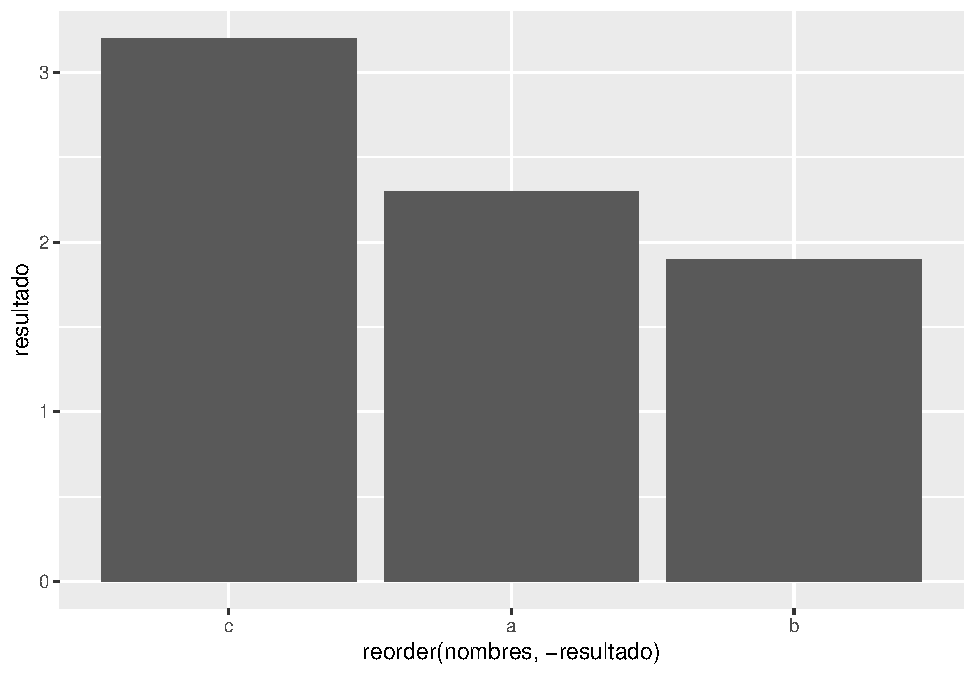
\includegraphics{clase_visualizacion_CSC_files/figure-latex/unnamed-chunk-17-1.pdf}

  \bibliography{book.bib,packages.bib}

\end{document}
